\documentclass[14pt,a4paper]{scrartcl}
\usepackage{cmap}
\usepackage[utf8]{inputenc}
\usepackage[T1,T2A]{fontenc}
\usepackage[english,russian]{babel}
\usepackage{relsize}
\usepackage{graphicx}
\usepackage{subfigure}
\usepackage{mathtools}
\usepackage{amssymb}
\usepackage{float}
\usepackage{sidecap}
\usepackage{wrapfig}
\usepackage{caption}
\usepackage[table,xcdraw]{xcolor}
\usepackage{minted}
\begin{document}
	\begin{titlepage}
	\begin{center}
		\large
		МИНИСТЕРСТВО НАУКИ И ВЫСШЕГО ОБРАЗОВАНИЯ\\ РОССИЙСКОЙ ФЕДЕРАЦИИ
		
		\vspace{0.5cm}
		
		МГТУ им Н.Э.Баумана
		\vspace{0.25cm}
		
		Факультет ФН
		
		Кафедра вычислительной математики и математической физики
		\vfill
		
		
		Соколов Арсений Андреевич\\
		\vfill
		
		
		{\LARGE Домашнее задание №1 по теории случайных процессов\\[2mm]
		}
		\bigskip
		
		3 курс, группа ФН11-63Б\\
		Вариант 19
	\end{center}
	\vfill
	
	\newlength{\ML}
	\settowidth{\ML}{«\underline{\hspace{0.7cm}}» \underline{\hspace{2cm}}}
	\hfill\begin{minipage}{0.4\textwidth}
		Преподаватель\\
		\underline{\hspace{3cm}} Т.\,В.~Облакова\\
		«\underline{\hspace{0.7cm}}» \underline{\hspace{1.71cm}} 2019 г.
	\end{minipage}%
	\bigskip
	
	
	\vfill
	
	\begin{center}
		Москва, 2019 г.
	\end{center}
\end{titlepage}

\section*{Начальные данные}

\begin{minted}{R}
> ### Начальные данные:
> m <- 6 # Число состояний марковской цепи
> k <- 5 # время (шаги)
> n <- 180 # траектории
\end{minted}

\section*{Задание 1}

Смоделировать вектор начальных вероятностей $\vec{p(0)} = p(0)$ и матрицу переходных вероятностей $P$ для однородной цепи Маркова с данным числом состояний ${s_1,s_2,…,s_m}$.\\
\textbf{Решение.}\\
1. Генерируем $(m+1)$ раз вектор $\vec{r}=(r_1,r_2,…,r_{m-1})$ из независимых и равномерно распределенных на отрезке $[0,1]$ случайных величин.
\begin{minted}{R}
> r_tmp <- replicate((m+1), runif((m-1), min = 0, max = 1), 
+	simplify = F)
> r_tmp
[[1]]
[1] 0.45066371 0.72262666 0.42050214 0.06783483 0.88320485

[[2]]
[1] 0.8242142 0.7617941 0.7539623 0.3366703 0.3043498

[[3]]
[1] 0.2185084 0.5359067 0.8582141 0.5830969 0.8235462

[[4]]
[1] 0.8423917 0.3508982 0.7679280 0.7678528 0.5647737

[[5]]
[1] 0.9639266243 0.0453068030 0.3141512477 0.1360417465 0.0002298534

[[6]]
[1] 0.1153282 0.9037961 0.4722757 0.6230641 0.7023776

[[7]]
[1] 0.04486402 0.03884641 0.43333865 0.36851324 0.04714968
\end{minted}


2. Для каждого из полученных векторов строим вариационный ряд, то есть упорядочиваем по возрастанию.

\begin{minted}{R}
> r <- lapply(r_tmp, sort)
> r
[[1]]
[1] 0.06783483 0.42050214 0.45066371 0.72262666 0.88320485

[[2]]
[1] 0.3043498 0.3366703 0.7539623 0.7617941 0.8242142

[[3]]
[1] 0.2185084 0.5359067 0.5830969 0.8235462 0.8582141

[[4]]
[1] 0.3508982 0.5647737 0.7678528 0.7679280 0.8423917

[[5]]
[1] 0.0002298534 0.0453068030 0.1360417465 0.3141512477 0.9639266243

[[6]]
[1] 0.1153282 0.4722757 0.6230641 0.7023776 0.9037961

[[7]]
[1] 0.03884641 0.04486402 0.04714968 0.36851324 0.43333865
\end{minted}

3. Находим длины отрезков, на которые вектор $\vec{r}$ разбивает отрезок $[0;1]$ -- получаем вектор вероятностей $\vec{p}$.

\begin{minted}{R}
> p_tmp <- lapply(r, diff)
> 
> heads <- lapply(r, head, 1)
> tails <- lapply(r, function(x) (1-tail(x,1)))
> 
> p <- mapply(append, mapply(append, heads,p_tmp,SIMPLIFY = F),
+             tails, SIMPLIFY = F)
> p
[[1]]
[1] 0.067835 0.352667 0.030162 0.271963 0.160578 0.116795

[[2]]
[1] 0.3043498 0.0323205 0.4172920 0.0078317 0.0624201 0.1757858

[[3]]
[1] 0.218508 0.317398 0.047190 0.240449 0.034668 0.141786

[[4]]
[1] 3.5090e-01 2.1388e-01 2.0308e-01 7.5209e-05 7.4464e-02 1.5761e-01

[[5]]
[1] 0.00022985 0.04507695 0.09073494 0.17810950 0.64977538 0.03607338

[[6]]
[1] 0.115328 0.356947 0.150788 0.079314 0.201418 0.096204

[[7]]
[1] 0.0388464 0.0060176 0.0022857 0.3213636 0.0648254 0.5666614
\end{minted}

Проверим, что полученные вектора обладают свойством стохастичности:

\begin{minted}{R}
> mapply(sum, p)
[1] 1 1 1 1 1 1 1
\end{minted}

Получили, что сумма элементов каждого вектора $\vec{p}$ равна единице.

4. Первый из полученных векторов $\vec{p}$ считаем вектором начальных вероятностей, из остальных составляем матрицу переходов $P$, записывая их по строкам.

\begin{minted}{R}
> p0 <- p[[1]] # вектор начальных условий
> p0
[1] 0.06783483 0.35266731 0.03016157 0.27196295 0.16057819 0.11679515
> P <- t(simplify2array(p))[-1,] # матрица переходов
> P
           [,1]      [,2]      [,3]       [,4]     [,5]     [,6]
[1,] 0.30434983 0.0323205 0.4172920 7.8317e-03 0.062420 0.175786
[2,] 0.21850839 0.3173983 0.0471902 2.4045e-01 0.034668 0.141786
[3,] 0.35089815 0.2138756 0.2030791 7.5209e-05 0.074464 0.157608
[4,] 0.00022985 0.0450769 0.0907349 1.7811e-01 0.649775 0.036073
[5,] 0.11532824 0.3569474 0.1507884 7.9314e-02 0.201418 0.096204
[6,] 0.03884641 0.0060176 0.0022857 3.2136e-01 0.064825 0.566661
\end{minted}

\pagebreak
\section*{Задание 2}
Построить размеченный граф состояний цепи.\\
\textbf{Решение.}\\

\begin{minted}{R}
> library(markovchain)
> library(diagram)
> 
> png(filename = "../img/1.png",
+     width = 1920, height = 1080,
+     res = 96 * 1.25)
> plotmat(signif(P,3), 
+         lwd = 1, box.lwd = 2, 
+         cex.txt = 0.8, 
+         box.size = 0.04, 
+         box.type = "circle", 
+         box.prop = 0.5,
+         box.col = "light blue",
+         arr.length=.25,
+         arr.width=.1,
+         self.cex = .7,
+         self.shifty = -.01,
+         self.shiftx = .07,
+         main = "Markov Chain")
> dev.off()
\end{minted}

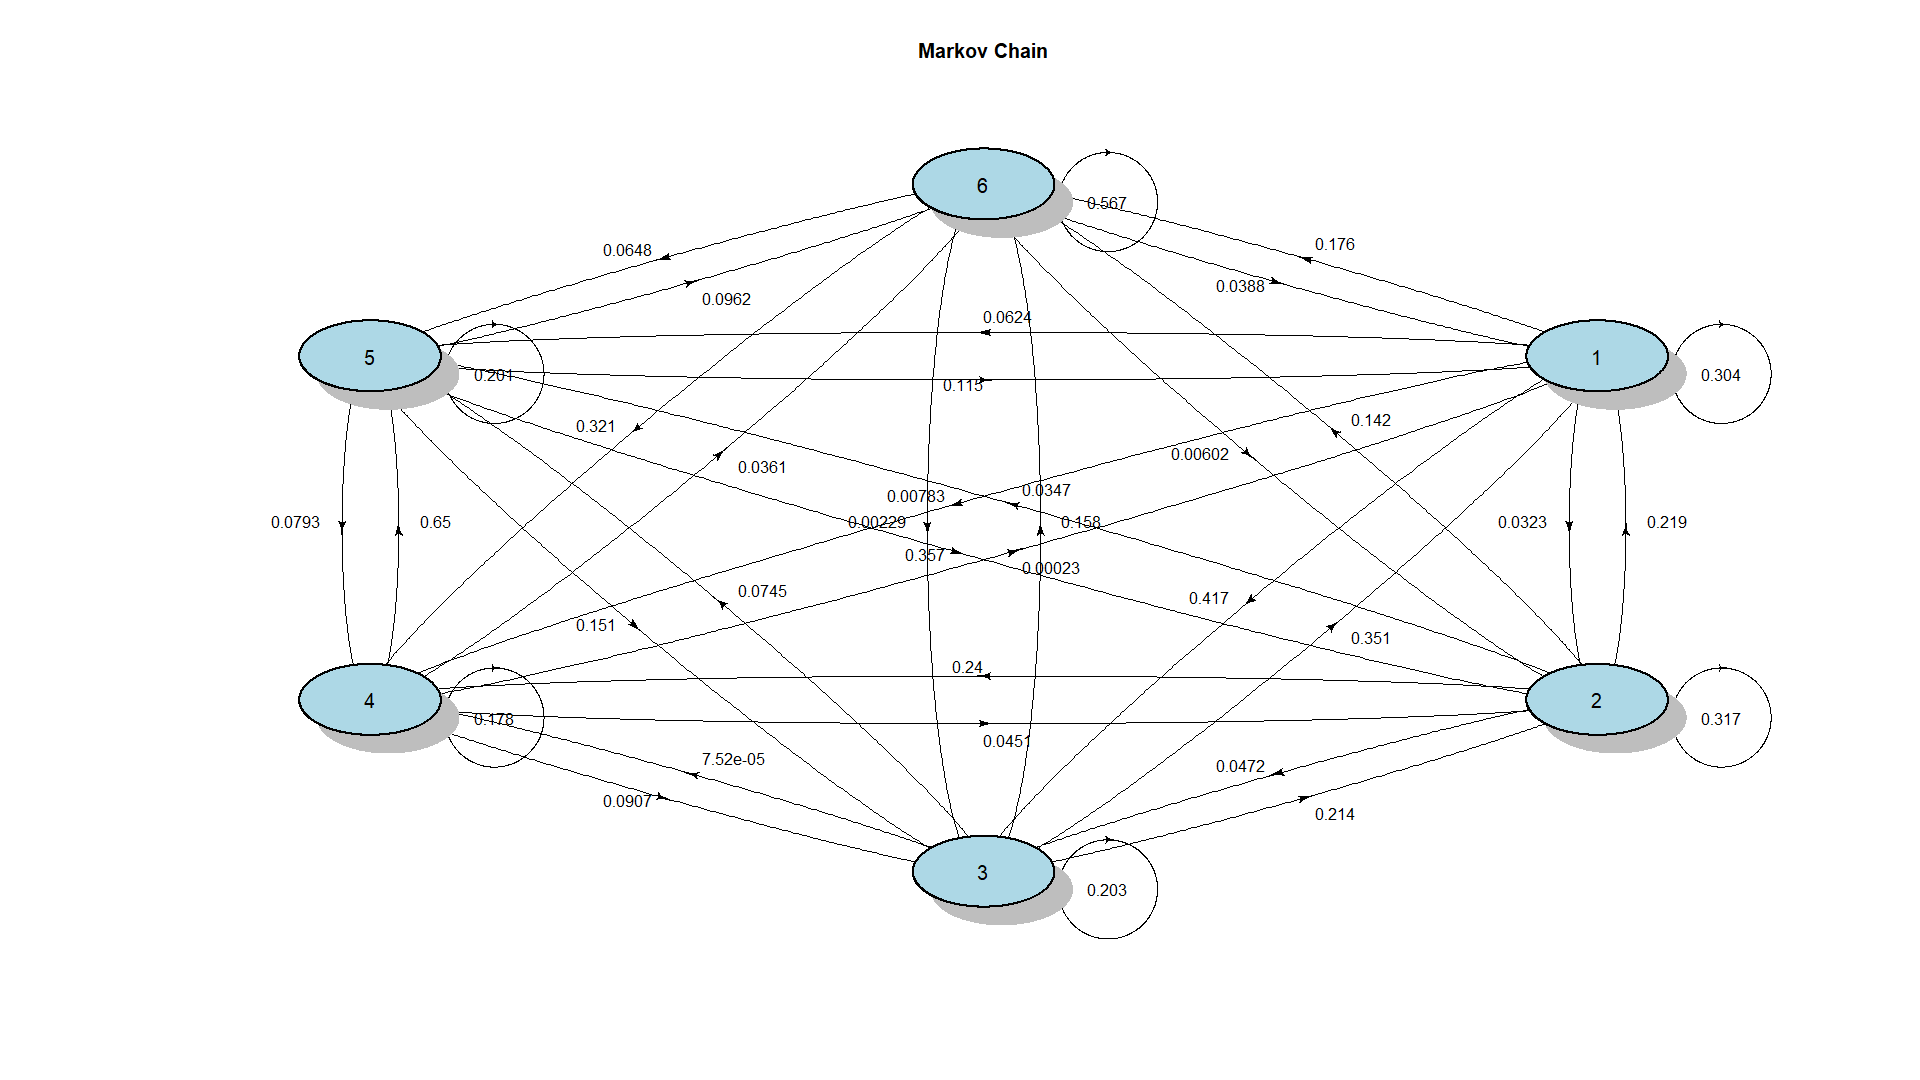
\includegraphics[angle=90,origin=t, scale=0.75]{../img/1.png}

\pagebreak

\section*{Задание 3.}
Вычислить безусловные вероятности состояний смоделированной цепи на k шаге.\\
\textbf{Решение.}\\

\begin{minted}{R}
> library(matrixcalc)
> p_k <- p0 %*% matrix.power(P,k)
> p_k
	[,1]      [,2]      [,3]      [,4]     [,5]      [,6]
[1,] 0.1640754 0.1558242 0.1454201 0.1477368 0.170361 0.2165826
\end{minted}


\section*{Задание 4}
Смоделировать $n$ траекторий полученной цепи за $k$ шагов и найти вектор относительных частот ее состояний на $k$ шаге.\\
\textbf{Решение.}\\

1. Генерируем равномерно распределенную на $[0;1]$ случайную величину $r_0$ и по вектору $\vec{r_1}$ разыгрываем начальное состояние следующим образом: если $r_0 < r_{1_1}$, то полагаем, что $\xi_0 = s_1 = 1$, если $r_0 < r_{1_2}$, то полагаем, что $\xi_0 = s_2 = 2$, \ldots, если $r_0 < r_{1_{m-1}}$, то полагаем, что $\xi_0 = s_{m-1} = m-1$, иначе если $r_0 > r_{1_{m-1}}$, то полагаем, что $\xi_0 = s_{m} = m = j_0$.


\begin{minted}{R}
> r0 <- runif(1, min = 0, max = 1)
> r0
[1] 0.3278443
> foo <- function(r0_loc,j)
+   {
+     ifelse(r0_loc < r[[j+1]][1],1,
+     ifelse(r0_loc < r[[j+1]][2],2,
+     ifelse(r0_loc < r[[j+1]][3],3,
+     ifelse(r0_loc < r[[j+1]][4],4,
+     ifelse(r0_loc < r[[j+1]][5],5,6)))))
+   }
>   
>   step_1 <- foo(r0,1)
> step_1
[1] 2
###
> r[[1]]
[1] 0.06783483 0.42050214 0.45066371 0.72262666 0.88320485
\end{minted}

Разыгранное число $r_0 = 0.3278443$, что меньше, чем 2-эй элемент $r_1$, но больше, чем 1-эй, то есть $(0.06783483 = r_{1_1}) < 0.3278443 < (0.42050214 = r_{1_2})  \Rightarrow \xi_0 = 2$. \\

2. Генерируем ещё одно значение $r_1$ и по строке с номером $j_0 = 2$ аналогично предыдущему пункту разыгрываем значение $\xi_1:$

\begin{minted}{R}
> r_1 <- runif(1, min = 0, max = 1)
> r_1
[1] 0.832978
> step_2 <- foo(r_1,step_1)
> step_2
[1] 5
\end{minted}

3. Повторяем алгоритм  заданное число раз $k$.

\begin{minted}{R}
> r_2 <- runif(1, min = 0, max = 1)
> r_2
[1] 0.4962721
> step_3 <- foo(r_2,step_2)
> step_3
[1] 3

> r_3 <- runif(1, min = 0, max = 1)
> r_3
[1] 0.3298892
> step_4 <- foo(r_3,step_3)
> step_4
[1] 1

> r_4 <- runif(1, min = 0, max = 1)
> r_4
[1] 0.4262919
> step_5 <- foo(r_4,step_4)
> step_5
[1] 3
\end{minted}

Получаем выборочную траекторию цепи:

\begin{minted}{R}
> c(step_1,step_2,step_3,step_4,step_5)
[1] 2 5 3 1 3
\end{minted}
	
4. Повторяем процедуру 1-3 $n$ число раз.

Полученный выше вектор подробно описан для одной итерации. В общем виде алгоритм выглядит, как представлено ниже в листинге. Очевидно, что вектор из предыдущего пункта не является первым вектором в получаемом ниже списке траекторий, так как алгоритм имеет общей вид.
\begin{minted}{R}
tracs <- list()

for (i in 1:n)
{
r0 <- runif(1, min = 0, max = 1)
foo <- function(r0_loc,j)
{
ifelse(r0_loc < r[[j+1]][1],1,
ifelse(r0_loc < r[[j+1]][2],2,
ifelse(r0_loc < r[[j+1]][3],3,
ifelse(r0_loc < r[[j+1]][4],4,
ifelse(r0_loc < r[[j+1]][5],5,6)))))
}

step_1 <- foo(r0,0)
step_2 <- foo(runif(1, min = 0, max = 1),step_1)
step_3 <- foo(runif(1, min = 0, max = 1),step_2)
step_4 <- foo(runif(1, min = 0, max = 1),step_3)
step_5 <- foo(runif(1, min = 0, max = 1),step_4)

trac <- list(c(step_1,step_2,step_3,step_4,step_5))
tracs[k] <- trac
}

tracs_array <- t(simplify2array(tracs,higher = F))
colnames(tracs_array) <- paste("Шаг",as.character(1:k))
rownames(tracs_array) <- paste("Тр.",as.character(1:n))
\end{minted}

В итоге получаем $n=180$ штук траекторий длины $k=5$.

Посмотрим на первые и последние 10 траекторий:

\begin{minted}{R}
> head(tracs_array,10)
	Шаг 1 Шаг 2 Шаг 3 Шаг 4 Шаг 5
Тр. 1      4     2     4     5     2
Тр. 2      5     2     2     4     6
Тр. 3      5     2     3     1     3
Тр. 4      2     4     5     5     5
Тр. 5      5     2     4     5     3
Тр. 6      6     4     3     6     4
Тр. 7      3     1     5     3     1
Тр. 8      2     6     6     4     5
Тр. 9      2     6     4     5     1
Тр. 10     2     2     6     6     6
> tail(tracs_array,10)
	Шаг 1 Шаг 2 Шаг 3 Шаг 4 Шаг 5
Тр. 171     2     1     3     2     2
Тр. 172     5     4     5     5     5
Тр. 173     5     2     4     5     2
Тр. 174     2     1     6     6     4
Тр. 175     1     1     1     3     3
Тр. 176     2     2     2     2     4
Тр. 177     5     2     6     5     6
Тр. 178     5     5     2     1     1
Тр. 179     2     2     6     6     6
Тр. 180     4     2     1     3     6
\end{minted}



\section*{Задание 5}
Вычислить эмпирические вероятности (относительные частоты) состояний  цепи на $k$ шаге.\\
\textbf{Решение.}\\

\begin{minted}{R}
> emp <- hist(tracs_array, breaks = 0:m)$density
> emp
[1] 0.1422222 0.1988889 0.1088889 0.1955556 0.1866667 0.1677778
\end{minted}

Сравним полученные эмпирические вероятности с вектором $\vec{p_k}$, полученным в 3 пункте. Для этого построим группированные bar-plots:

\begin{minted}{R}
> theor <- as.numeric(p_k)
> 
> 
> plot_df <- data.frame(type = rep(c("theoretical", "emperical"), each=m),
+                       step = rep(paste("Шаг",as.character(1:m)), 2),
+                       prob = c(theor, emp))
> 
> png(filename = "../img/2.png",
+     width = 1920, height = 1080,
+     res = 96 * 1.25)
> ggplot(data=plot_df, aes(x=step, y=prob, fill=type)) +
+   geom_bar(stat="identity", position=position_dodge()) + 
+   theme_bw()
> dev.off()
\end{minted}

\begin{figure}[H]
	\begin{minipage}[h]{1\linewidth}
		\center{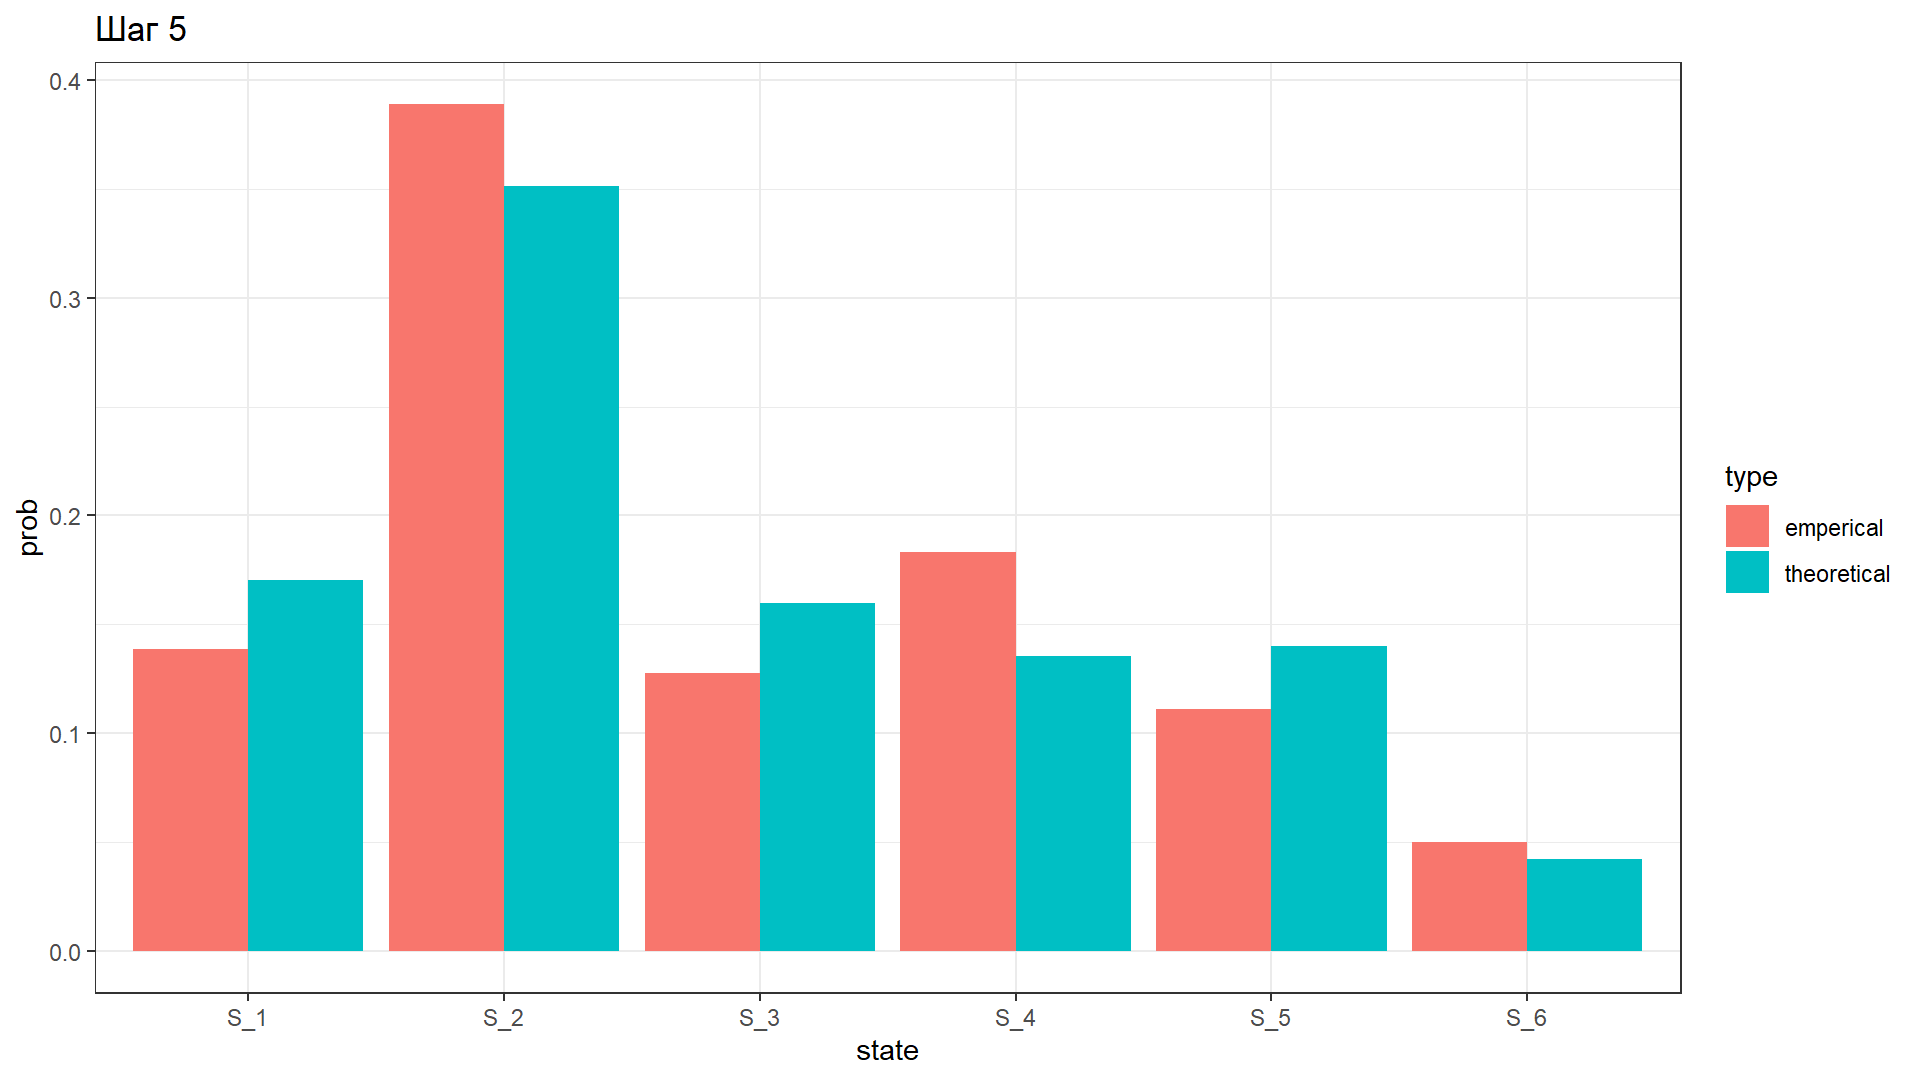
\includegraphics[width=1\linewidth]{../img/2.png}}  \\
	\end{minipage}
\end{figure}


Рассмотрим разности соответствующих значений эмпирической и теоретической вероятностей, а также максимальное по модулю значение разности:

\begin{minted}{R}
> prob_diff <- emp - theor
> prob_diff
[1] -0.02185318  0.04306471 -0.03653119  0.04781875  0.01630567 -0.04880477
> max(abs(prob_diff))
[1] 0.04880477
\end{minted}


\section*{Задание 6}
Вычислить финальные вероятности для марковской цепи и сравнить их  вероятностями состояний на $k$ шаге.\\
\textbf{Решение.}\\

Для нахождения финальных вероятностей марковской цепи рассмотрим систему:
\begin{equation*}
	\begin{cases} 
		\sum\limits_{i=1}^m \pi_i P_{i,j} = \pi_j\\ 
		\sum\limits_{i=1}^m \pi_i = 1\\ 
	\end{cases}
\end{equation*}



\end{document}